\documentclass{article}
% generated by Madoko, version 1.1.3
%mdk-data-line={1}


\usepackage[heading-base={2},section-num={False},bib-label={hide},fontspec={True}]{madoko2}


\begin{document}



%mdk-data-line={5}
\mdxtitleblockstart{}
%mdk-data-line={5}
\mdxtitle{\mdline{5}Angel调研及使用报告}%mdk
\mdxauthorstart{}
%mdk-data-line={10}
\mdxauthorname{\mdline{10}ryanyycao(曹洋毓)}%mdk
\mdxauthorend\mdtitleauthorrunning{}{}\mdxtitleblockend%mdk

%mdk-data-line={7}
\section{\mdline{7}1.\hspace*{0.5em}\mdline{7}综述}\label{section}%mdk%mdk

%mdk-data-line={9}
\noindent\mdline{9}\hspace*{1em}\mdline{9}\hspace*{1em}\mdline{9}Angel是一个基于参数服务器的高性能分布式机器学习平台,核心设计理念围绕机器学习模型,将高维度的大模型合理切分到多个参数服务器节点。
Angel的主要核心抽象是PSModel,它将对分布于多台PS Server上的远程模型操作透明化,通过PSModel,用户可以方便的进行模型的更新,
自定义函数计算,以及同步控制,从而实现各种高效的机器学习算法。Angel基于Java和Scala进行开发,可以使用Yarn直接调度运行,并且支持
Spark on Angel%mdk

%mdk-data-line={14}
\section{\mdline{14}2.\hspace*{0.5em}\mdline{14}架构设计}\label{section}%mdk%mdk

%mdk-data-line={15}
\subsection{\mdline{15}2.1.\hspace*{0.5em}\mdline{15}Angel中的各种角色:}\label{sec-angel}%mdk%mdk

%mdk-data-line={18}
\begin{mddefinitions}%mdk

\mddefterm{\noindent{\bfseries Client}}%mdk

%mdk-data-line={18}
\begin{mdbmarginx}{}{}{}{1.5em}%mdk
\begin{mddefdata}%mdk
\mdline{18}\hspace*{1em}\mdline{18}\hspace*{1em}\mdline{18}控制任务运行,启动和停止Angel任务,加载和存储模型,启动具体计算过程和获取任务运行状态等
%mdk
\end{mddefdata}%mdk
\end{mdbmarginx}%mdk

\mddefterm{\noindent{\bfseries Master}}%mdk

%mdk-data-line={20}
\begin{mdbmarginx}{}{}{}{1.5em}%mdk
\begin{mddefdata}%mdk
\mdline{20}\hspace*{1em}\mdline{20}\hspace*{1em}\mdline{20}原始计算数据以及参数矩阵的分片和分发,申请Worker和ParameterServer所需的计算资源,协调,管理和监控Worker以及ParameterServer
%mdk
\end{mddefdata}%mdk
\end{mdbmarginx}%mdk

\mddefterm{\noindent{\bfseries Parameter Server}}%mdk

%mdk-data-line={22}
\begin{mdbmarginx}{}{}{}{1.5em}%mdk
\begin{mddefdata}%mdk
\mdline{22}\hspace*{1em}\mdline{22}\hspace*{1em}\mdline{22}负责存储和更新参数
%mdk
\end{mddefdata}%mdk
\end{mdbmarginx}%mdk

\mddefterm{\noindent{\bfseries Worker}}%mdk

%mdk-data-line={24}
\begin{mdbmarginx}{}{}{}{1.5em}%mdk
\begin{mddefdata}%mdk
\mdline{24}\hspace*{1em}\mdline{24}\hspace*{1em}\mdline{24}负责具体的模型训练或者结果预测,一个计算任务往往包含许多个Worker实例,每个Worker实例负责使用一部分训练数据进行训练%mdk
\end{mddefdata}%mdk
\end{mdbmarginx}%mdk
%mdk
\end{mddefinitions}%mdk

%mdk-data-line={26}
\noindent\mdline{26}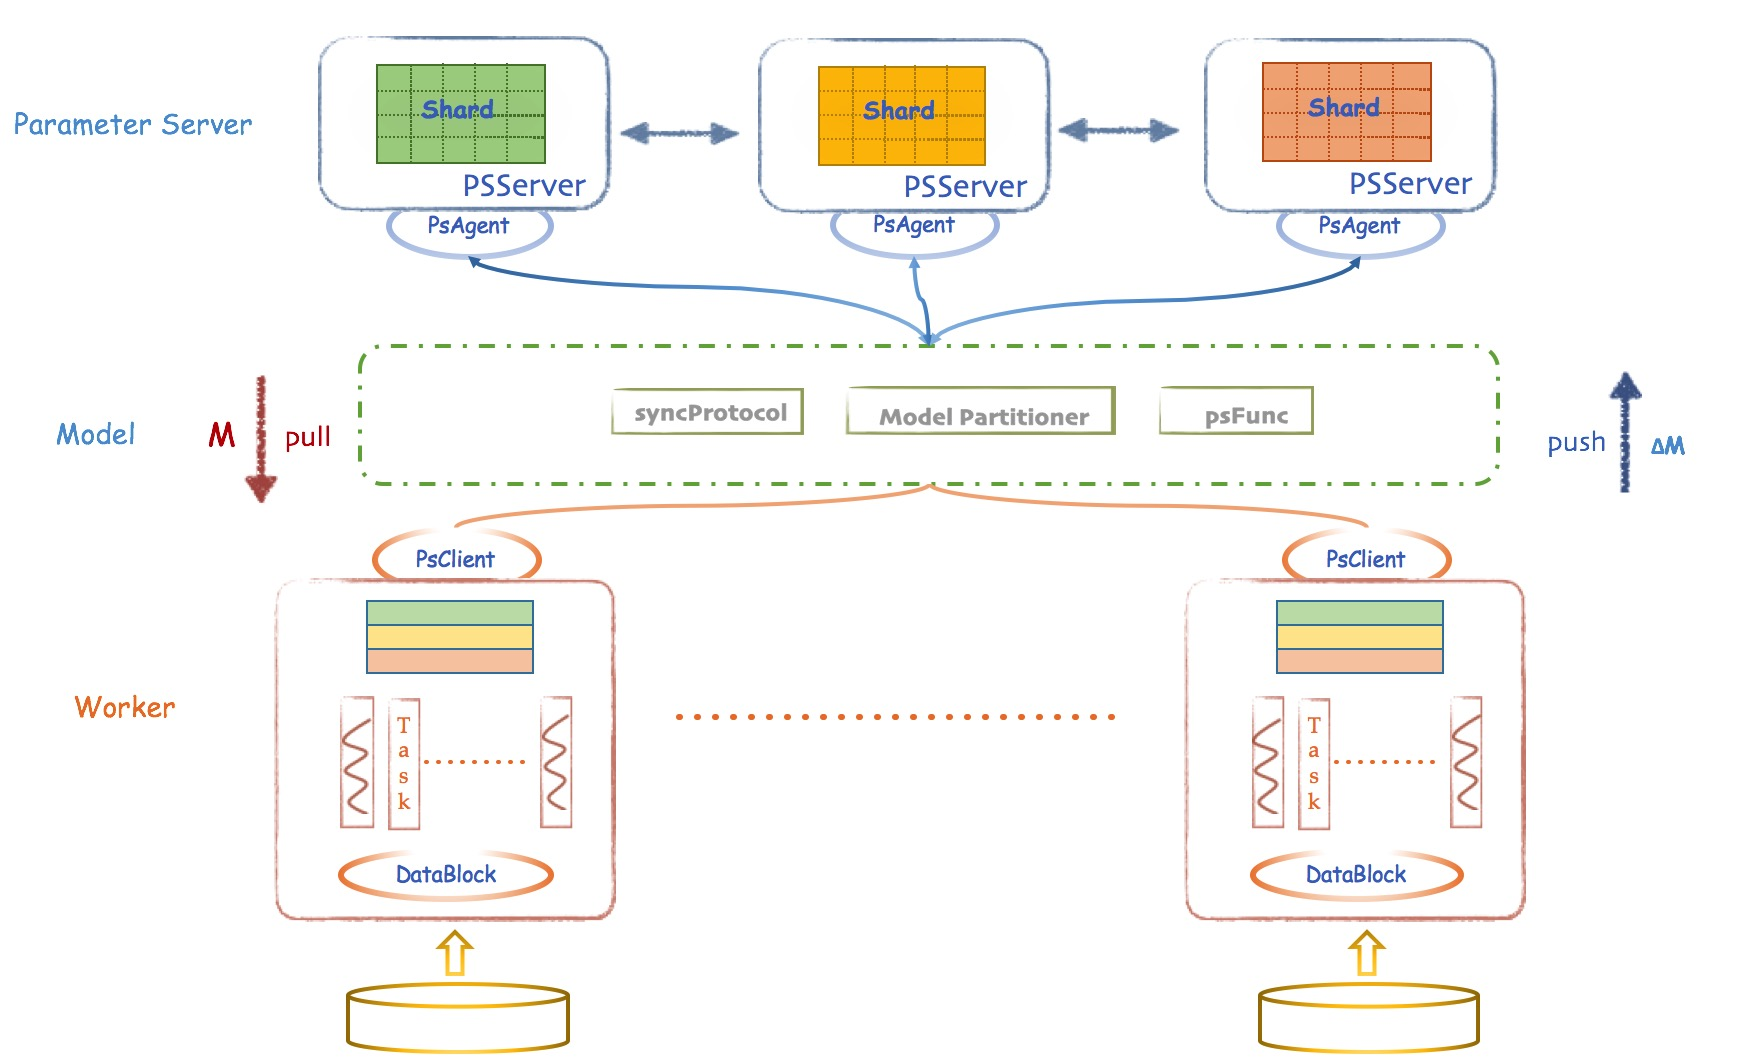
\includegraphics[keepaspectratio=true,width=\dimmin{}{\dimwidth{0.90}}]{images/angel_architecture_1}{}\mdline{26}
\mdline{27} \mdline{27}%mdk

%mdk-data-line={30}
\subsection{\mdline{30}2.2.\hspace*{0.5em}\mdline{30}Angel中的核心抽象:}\label{sec-angel}%mdk%mdk

%mdk-data-line={32}
\begin{mddefinitions}%mdk

\mddefterm{\noindent{\bfseries PSModel}}%mdk

%mdk-data-line={32}
\begin{mdbmarginx}{}{}{}{1.5em}%mdk
\begin{mddefdata}%mdk
\mdline{32}\hspace*{1em}\mdline{32}\hspace*{1em}\mdline{32}PSModel是一个远程模型的概念,对于Client来说,它是一个类似模型代理的类。通过它你可以在每个Worker上,像操作本地对象一样去操作一个模型,而实际上你操作的是一个均匀切分在远程多个PSServer上的分布式模型切片,而且所有的操作都是透明并发的
%mdk
\end{mddefdata}%mdk
\end{mdbmarginx}%mdk

\mddefterm{\noindent{\bfseries MLModel}}%mdk

%mdk-data-line={34}
\begin{mdbmarginx}{}{}{}{1.5em}%mdk
\begin{mddefdata}%mdk
\mdline{34}\hspace*{1em}\mdline{34}\hspace*{1em}\mdline{34}由一系列的PSModel(远程模型)构成,对这些模型进行统一操作%mdk
\end{mddefdata}%mdk
\end{mdbmarginx}%mdk
%mdk
\end{mddefinitions}%mdk

%mdk-data-line={37}
\section{\mdline{37}3.\hspace*{0.5em}\mdline{37}高级特性}\label{section}%mdk%mdk

%mdk-data-line={39}
\subsection{\mdline{39}3.1.\hspace*{0.5em}\mdline{39}多种参数同步协议(通过向量时钟实现)}\label{section}%mdk%mdk

%mdk-data-line={40}
\begin{itemize}[noitemsep,topsep=\mdcompacttopsep]%mdk

%mdk-data-line={40}
\item{}
%mdk-data-line={40}
\mdline{40}BSP:在每一轮迭代中都需要等待所有的Task计算完成%mdk%mdk

%mdk-data-line={42}
\item{}
%mdk-data-line={42}
\mdline{42}SSP:允许一定程度的Task进度不一致,但这个不一致有一个上限%mdk%mdk

%mdk-data-line={44}
\item\mdline{44}ASP:Task之间完全不用相互等待,先完成的Task,继续下一轮的训练%mdk
%mdk
\end{itemize}%mdk

%mdk-data-line={46}
\subsection{\mdline{46}3.2.\hspace*{0.5em}\mdline{46}ps function(psf)}\label{sec-ps-functionpsf}%mdk%mdk

%mdk-data-line={47}
\noindent\mdline{47}  \mdline{47}\hspace*{1em}\mdline{47}\hspace*{1em}\mdline{47}通过继承Angel提供的psf函数接口,可以实现自己的参数获取/更新逻辑,在不修改Angel自身代码的情况下定制自己想要的参数服务器的接口%mdk

%mdk-data-line={49}
\begin{itemize}[noitemsep,topsep=\mdcompacttopsep]%mdk

%mdk-data-line={49}
\item\mdline{49}设计理念:实际应用中,各个算法对参数服务器上的参数获取和更新,远远不只pull()/push()这么简单,尤其是当算法需要实施一些特定的优化的时候。
psf可以支持在ps端做一些简单的计算,从而在计算开销不变的情况下降低通信开销%mdk

%mdk-data-line={51}
\item{}
%mdk-data-line={51}
\mdline{51}整体架构%mdk

%mdk-data-line={53}
\mdline{53}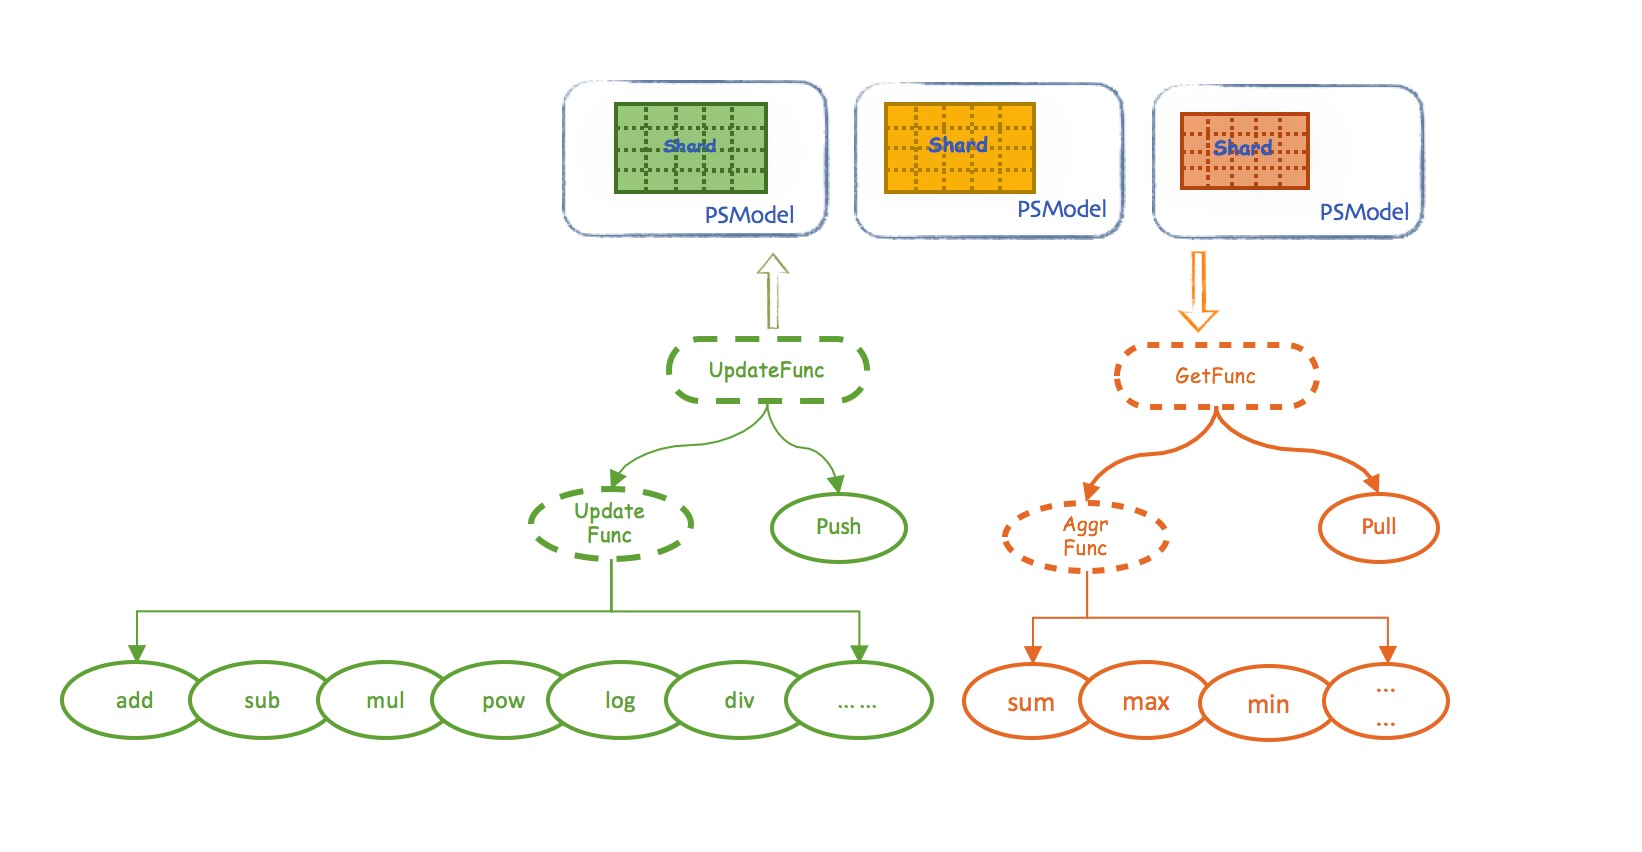
\includegraphics[keepaspectratio=true,width=\dimmin{}{\dimwidth{0.90}}]{images/angel_psFunc}{}\mdline{53}%mdk%mdk

%mdk-data-line={55}
\item{}
%mdk-data-line={55}
\mdline{55}GetFunc(参数获取)%mdk

%mdk-data-line={57}
\mdline{57}请求划分:操作的是整个模型参数,进行请求划分,生成一个请求列表,这个请求列表中,每一个请求都和一个模型参数分区对应%mdk

%mdk-data-line={59}
\mdline{59}请求发送:将请求列表中的所有请求,发送给模型参数分区所在的PSServer,PSServer以模型参数分区为单位执行参数获取和更新操作,并返回相应的结果%mdk

%mdk-data-line={61}
\mdline{61}请求合并:合并所有的模型分区级结果,得到最终的结果并返回%mdk%mdk

%mdk-data-line={63}
\item{}
%mdk-data-line={63}
\mdline{63}UpdateFunc(参数更新)%mdk

%mdk-data-line={65}
\mdline{65}请求划分:PSClient进行请求划分,生成一个请求列表,这个请求列表中的每一个请求都和一个模型参数分区对应%mdk

%mdk-data-line={67}
\mdline{67}请求发送:将请求列表中的所有请求发送给模型参数分区所在的PS实例,PS实例以模型参数分区为单位执行更新操作%mdk

%mdk-data-line={69}
\mdline{69}等待完成:等待所有请求完成后返回%mdk

%mdk-data-line={71}
%mdk-data-line={72}
\noindent\mdline{72}\textbf{Note}.
\mdline{73}无论是Get还是Update,具体的这三个阶段,其过程都是可以自定义的,从而实现千变万化的psFunc。%mdk%mdk

%mdk-data-line={74}
%mdk-data-line={75}
\noindent\mdline{75}\textbf{Note}.
\mdline{76}之前github相关文档中提到psf分为client-ps的psf和ps-ps的psf,后联系作者确认并没有ps-ps的psf,github文档有误。%mdk%mdk%mdk
%mdk
\end{itemize}%mdk

%mdk-data-line={82}
\subsection{\mdline{82}3.3.\hspace*{0.5em}\mdline{82}自定义模型切片}\label{section}%mdk%mdk

%mdk-data-line={84}
\begin{itemize}[noitemsep,topsep=\mdcompacttopsep]%mdk

%mdk-data-line={84}
\item\mdline{84}Angel默认的模型分区:将模型切分成大小相等的矩形区域。1)尽量将一个模型平均分配到所有PS节点上;2)对于非常小的模型,将它们尽量放在一个PS节点上;3)对于多行的模型,尽量将同一行放在一个PS节点上%mdk

%mdk-data-line={85}
\item\mdline{85}自定义模型分区:设置自定义的Partitioner,实现两个接口getPartitions和assignPartToServer,最后将其将其注入到PSModel的MatrixContext之中即可使用

%mdk-data-line={86}
\subsection{\mdline{86}3.4.\hspace*{0.5em}\mdline{86}支持多种容错}\label{section}%mdk%mdk%mdk

%mdk-data-line={87}
\item\mdline{87}PS容错采用了checkpoint的模式%mdk

%mdk-data-line={88}
\item\mdline{88}挂掉的Worker实例可以从Master处获取当前迭代轮数等状态信息,从PS处获取最新模型参数,然后重新开始被断掉的迭代%mdk

%mdk-data-line={89}
\item\mdline{89}Master定期将任务状态写入hdfs,挂掉后Yarn会重新拉起一个Angel的Master,加载状态信息,重新启动Worker和PS,从断点处重新开始计算。%mdk
%mdk
\end{itemize}%mdk

%mdk-data-line={91}
\section{\mdline{91}4.\hspace*{0.5em}\mdline{91}Angel编译和运行}\label{sec-angel}%mdk%mdk

%mdk-data-line={93}
\begin{itemize}[noitemsep,topsep=\mdcompacttopsep]%mdk

%mdk-data-line={93}
\item\mdline{93}环境要求:Jdk \mdline{93}\textgreater{}\mdline{93}= 1.8 Maven \mdline{93}\textgreater{}\mdline{93}= 3.0.5 Protobuf \mdline{93}\textgreater{}\mdline{93}= 2.5.0且和Hadoop的Protobuf版本一致%mdk

%mdk-data-line={94}
\item\mdline{94}源码下载:git clone https://github.com/Tencent/angel%mdk

%mdk-data-line={95}
\item\mdline{95}编译:mvn clean package\mdline{95} \mdline{95}-Dmaven.test.skip=true  发布包位于dist/target目录下%mdk

%mdk-data-line={96}
\item\mdline{96}运行时可以选择本地运行,或通过Yarn提交到集群运行

%mdk-data-line={97}
%mdk-data-line={98}
\noindent\mdline{98}\textbf{Note}.
\mdline{99}由于Angel编译要求和Hadoop的Protobuf版本一致,中心集群Hadoop的Protobuf版本为2.4,
而Angel使用Protobuf2.4会报很多方法没有实现的错误,需要修改很多底层源码,暂时来看在中心集群搭建分布式Angel不可行%mdk%mdk%mdk
%mdk
\end{itemize}%mdk

%mdk-data-line={102}
\section{\mdline{102}5.\hspace*{0.5em}\mdline{102}开发新算法过程}\label{section}%mdk%mdk

%mdk-data-line={104}
\begin{enumerate}[noitemsep,topsep=\mdcompacttopsep]%mdk

%mdk-data-line={104}
\item\mdline{104}定义一个模型,继承MLModel,里面定义参数模型及其他的一些配置%mdk

%mdk-data-line={105}
\item\mdline{105}定义一个Task,继承自TrainTask,定义模型的训练过程,需要实现parse()和train()两个方法,分别为解析数据和训练%mdk

%mdk-data-line={106}
\item\mdline{106}定义一个Runner,继承自MLRunner,用于将任务提交到集群,实现train()和predict()两个方法%mdk

%mdk-data-line={107}
\item\mdline{107}如果有定制化模型切片和psf的需求,还需要自定义模型切片方法和psf

%mdk-data-line={108}
%mdk-data-line={109}
\noindent\mdline{109}\textbf{Note}.
\mdline{110}之前准备基于Angel开发的Distributed Negative Sampling for Word Embeddings算法强依赖于ps-ps的psf,
现在发现Angel并不支持这种ps到ps通信的特性,基于Angel只能实现简单的Word2Vec算法,暂时放弃这个方案%mdk%mdk%mdk
%mdk
\end{enumerate}%mdk

%mdk-data-line={113}
\section{\mdline{113}6.\hspace*{0.5em}\mdline{113}总结}\label{section}%mdk%mdk

%mdk-data-line={114}
\noindent\mdline{114}\hspace*{1em}\mdline{114}\hspace*{1em}\mdline{114}通过这次基于Angel的实践,大概摸索到了Angel的能力范围。Angel核心抽象为模型,特色为将模型分布于多台PS Server,然后提供一整套的psf来对远程模型进行操作。
在支持了自定义模型分区策略、自定义client—ps的psf的高级特性之后,它的优势就很明显的体现了出来,这两个特性可以很好的安排模型的分布,安排计算的位置(client or ps),安排
通信内容,可以很明显的提升某些机器学习算法的性能(类似于之前实现的那种Word2Vec算法)。但是对于没有ps概念的算法来说,所有的节点之间需要进行通信,由于Angel不提供ps-ps的psf,因此没有办法
完成ps间的交互,因此开发这类算法比较困难。%mdk

%mdk-data-line={119}
\mdline{119}\hspace*{1em}\mdline{119}\hspace*{1em}\mdline{119}通过默认的模型分区策略,和自定义的模型分区策略,Angel的模型分区上,在方便性和灵活性,做出了很好的平衡,为用户实现高效的复杂算法,打下了良好的基础。%mdk

%mdk-data-line={121}
\mdline{121}\hspace*{1em}\mdline{121}\hspace*{1em}\mdline{121}随着psFunc的引入,模型的计算,也会发生在PSServer端。PSServer也将有一定的模型计算职责,而不是单纯的模型存储功能。合理的设计psFunc,将大大的加速算法的运行。
伴随着psFunc的引入和强化,在很多复杂的算法实现中,大大的降低了Worker要把模型完整的拖回来进行整体计算的可能性,从而曲线的实现了模型并行。%mdk%mdk


\end{document}
